\documentclass[solution, letterpaper]{cs121}

\usepackage{tikz-qtree}
\usepackage{graphicx}

%% Please fill in your name and collaboration statement here.
%\newcommand{\studentName}{Renzo Lucioni and Daniel Broudy}
%\newcommand{\collaborationStatement}{I collaborated with...}
\newcommand{\solncolor}{red}
\begin{document}

\header{1}{February 15, 2013, at 12:00 PM}{}{}

%%%%%%%%%%%%%%%%%%%%%%%%%%%%%%%%%%%%%%%%%%%%%%%%%%%%
\problem{15}
\subproblem The following are information gain calculations performed by the ID3 algorithm when deciding on which attribute, \emph{A} or \emph{B}, to split. First, we estimate the initial entry before splitting.

\[ H(\text{labels}) \approx \frac{4}{7} (\log_2 \frac{7}{4}) + \frac{3}{7} (\log_2 \frac{7}{3}) \approx 0.99 \]

Next, we calculate the specific conditional entropy of the labels given \emph{A} = 1.

\[ H(\text{labels } | \text{ } A = 1) \approx \frac{1}{2} (\log_2 2) + \frac{1}{2} (\log_2 2) = 1 \]

Then we compute the specific conditional entropy of the labels given \emph{A} = 0.

\[ H(\text{labels } | \text{ } A = 0) \approx \frac{2}{3} (\log_2 \frac{3}{2}) + \frac{1}{3} (\log_2 3) \approx 0.92 \]

Now we find the conditional entropy of the labels given that we split on \emph{A}.

\[ H(\text{labels } | \text{ } A) \approx \frac{4}{7}(1) + \frac{3}{7}(0.92) \approx 0.97 \]

Finally, we estimate the mutual information between \emph{A} and the labels.

\[ I(\text{labels } ; \text{ } A) \approx  0.99 - 0.97 \approx 0.02\]

Using the same procedure, we compute the information gain from splitting on \emph{B}.

\[ H(\text{labels } | \text{ } B = 1) \approx  \frac{1}{2} (\log_2 2) + \frac{1}{2} (\log_2 2) = 1 \]

\[ H(\text{labels } | \text{ } B = 0) \approx  \frac{3}{5} (\log_2 \frac{5}{3}) + \frac{2}{5} (\log_2 \frac{5}{2}) \approx 0.97 \]

\[ H(\text{labels } | \text{ } B) \approx \frac{2}{7}(1) + \frac{5}{7}(0.97) \approx 0.98 \]

\[ I(\text{labels } ; \text{ } B) \approx  0.99 - 0.98 \approx 0.01 \]

Now we compare the possible information gains. Since $0.02 > 0.01$, ID3 will decide to split on attribute \emph{A}.

One can argue that splitting on \emph{A} is more useful than splitting on \emph{B}, since it is the attribute associated with the highest local information gain (i.e., the entropy of the negative value is locally the lowest). However, one can also argue that splitting on \emph{B} is more useful than splitting on \emph{A}, since doing so allows for immediately labeling 3 of 7 instances as positive and giving  ``no information" on 2 instances, whereas splitting on \emph{A} allows for labeling only 2 of 7 instances as positive and giving ``no information" on 4 instances. This example shows that ID3 has a preference for trees with high information gain attributes near the root, simultaneously demonstrating the algorithm's preference for making the most extreme local partition possible.

\subproblem The following is a decision tree ID3 might construct for the given dataset.

\begin{center}
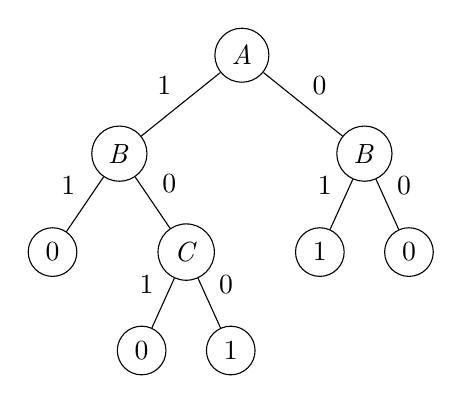
\begin{tikzpicture}[every tree node/.style={draw,circle},
   level distance=1.25cm,sibling distance=.5cm, 
   edge from parent path={(\tikzparentnode) -- (\tikzchildnode)}]
\Tree [.\node {\emph{A}}; 
    \edge node[auto=right] {1}; [.\emph{B}
      \edge node[auto=right] {1}; [.0 ] \edge node[auto=left] {0}; [.\emph{C} 
        \edge node[auto=right] {1}; [.0 ] \edge node[auto=left] {0}; [.1 ] 
      ]
    ]
    \edge node[auto=left] {0}; [.\emph{B}
      \edge node[auto=right] {1}; [.1 ] \edge node[auto=left] {0}; [.0 ]
    ] ]
\end{tikzpicture}
\end{center}

Attribute \emph{A} yields the highest information gain, so ID3 uses \emph{A} as the root of the tree. After arbitrarily breaking an information gain tie with \emph{C}, \emph{B} is chosen as the first node on the left. \emph{C} is chosen as the next node extending from \emph{B} because it fully explains the remaining data. After arbitrarily breaking an information gain tie with \emph{C}, \emph{B} is chosen as the first node on the right. At this point we see that we have inconsistent data but no features left to branch on, so we select the majority target to minimize the number of misclassified examples. The resulting tree misclassifies 1 of 7 examples, indicating that this classifier has an accuracy of $\frac{6}{7} \approx 0.86$.


\subproblem The following is a simpler tree that has the same training error as the one produced by ID3.

\begin{center}
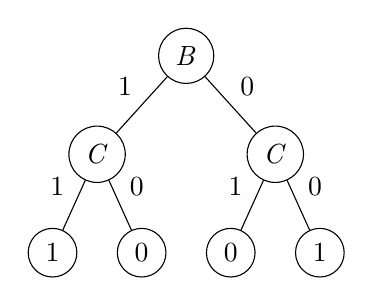
\begin{tikzpicture}[every tree node/.style={draw,circle},
   level distance=1.25cm,sibling distance=.5cm, 
   edge from parent path={(\tikzparentnode) -- (\tikzchildnode)}]
\Tree [.\node {\emph{B}}; 
    \edge node[auto=right] {1}; [.\emph{C}
      \edge node[auto=right] {1}; [.1 ] \edge node[auto=left] {0}; [.0 ]
    ]
    \edge node[auto=left] {0}; [.\emph{C}
      \edge node[auto=right] {1}; [.0 ] \edge node[auto=left] {0}; [.1 ]
    ] ]
\end{tikzpicture}
\end{center}

This tree also has accuracy 0.86. This example shows us that ID3 does not always build the simplest tree possible, but instead finds a ``good" tree which is an approximation of the simplest tree. More importantly, this example also teaches us that ID3 is unable to look ahead to see which attributes are good co-predictors. 

%%%%%%%%%%%%%%%%%%%%%%%%%%%%%%%%%%%%%%%%%%%%%%%%%%%%
\problem{25}
\subproblem The average cross-validated training performance over the ten trials for the non-noisy dataset is 1.0; the test performance is 0.87. The average cross-validated training performance over the ten trials for the noisy dataset is 0.98; the test performance is 0.78.
\pagebreak
\subproblem
 
(i) The requested graphs are below. 
\begin{center}
\includegraphics[scale=0.8]{prune-non-noisy.pdf}
\includegraphics[scale=0.8]{prune-noisy.pdf}
\end{center}

(ii) For both the non-noisy and noisy datasets, the cross-validated test performance (i.e., predictive accuracy) of the validation set pruning increases gradually as the size of the validation set goes from 0 to 50. The cross-validated test performance peaks for validation set sizes of approximately 50 (more precisely, 51 for the non-noisy data, and 55 for the noisy data). Then, as the size of the validation set approaches 80, cross-validated test performance decreases significantly while training performance increases, due to the fact that ID3 has much less data on which to train a decision tree (the size of the training dataset is approaching 10). \\

(iii) Yes, the validation set pruning improves the cross-validated performance of ID3 on these data. \emph{Without} validation set pruning, the average cross-validated test performance over ten trials for the non-noisy dataset is 0.87 (as stated above). With validation set pruning, the average cross-validated test performance over ten trials for the non-noisy dataset reaches 0.9 when the validation set size is 51 (1.0 training accuracy). For the noisy dataset, the average cross-validated test performance over ten trials improves from 0.78 without pruning to 0.84 with pruning when the validation set size is 55 (0.98 training accuracy). \\

(iv) Yes, overfitting is an issue for these data. The unpruned tree generated in 2(A) has high average cross-validated training performance over the ten trials on both the noisy and non-noisy datasets. As demonstrated in (iii), while pruning can negatively impact training performance by simplifying the tree, it improves average cross-validated test performance over ten trials for both datasets, suggesting that pruning helps the tree to generalize better. This implies that the original, unpruned tree was overfit, and that the simplified, pruned tree is less so. ({\bf NB:} In our implementation of pruning, we made the assumption that it should not be possible for a tree to be pruned all the way down to just a leaf; the smallest a tree can get in our implementation is a decision stump of depth 1.)

%%%%%%%%%%%%%%%%%%%%%%%%%%%%%%%%%%%%%%%%%%%%%%%%%%%%
\problem{30}
\subproblem In order to implement boosting, we must define an information gain criterion that takes example weights into account. We can do so by modifying ID3's definition of entropy given weights $w_n^{(r)}$ on the data. More specifically, we will weight the counts of instances in each class by the weight on the instance. That is, to find a weight for each class, we will sum the weights of the instances whose label matches the class. We will make a similar change to the method used to compute mutual information in problem (1). Namely, we replace all counts with sums of weights. As usual, we decide to split on the attribute with the highest weighted information gain.

In the given example set, the sum of all example weights is equal to 1. There is only one example with label 1, and its weight is 0.5. The other examples have label 0, so we sum their weights to get 0.5 total. Therefore, the weighted entropy of the given set is
\[ H(\mathcal D) \approx \frac{.5}{1} (\log_2 \frac{1}{0.5}) + \frac{.5}{1} (\log_2 \frac{1}{0.5}) = 1 \]


\subproblem

(i)  As we increase the max depth the test performance for boosting goes down. This is probably due to issues of over fitting, if we enforce a shallower depth our weak learners don't fit as strictly to the noisy training data increasing performance on the test data. 
 We can explain the below results as a demonstration of this phenomenon. As you increase the depth of the boosting trees you allow them to fit more closely to the noisy data. If you look at the table with 30 rounds on the noisy data set, you can see that allowing a depth of 2 actually caused the cross-validated test performance to suffer. 
 
\begin{center}
\begin{tabular}{| l | c r |  l | c r | }    
\hline
      \multicolumn{3}{| c | }{Non-Noisy} & \multicolumn{3}{| c | }{Noisy}  \\    \hline         
       &\multicolumn{2}{c |}{depth} &  &\multicolumn{2}{c |}{depth} \\             
   rounds & 1 & 2 &    rounds& 1 & 2  \\ \hline
  10 & .93 & .9 & 10 & .83 & .84 \\
  30 & .94 & .93 & 30 & .83 & .79 \\
\hline
           
\end{tabular}
\end{center}

(ii) The requested graphs are below. For both, the depth of the weak learners is fixed at 1.
\begin{center}
\includegraphics[scale=0.8]{boost-non-noisy.pdf}
\includegraphics[scale=0.8]{boosted-noisy.pdf}
\end{center}
As the number of boosting rounds increases, the training and test accuracy improve. This is true for both the non-noisy and the noisy data sets. When run on the non-noisy data set, test accuracy continues to improve for a while even after training accuracy reaches 1.0 (i.e., training error has gone to 0). This is expected based on our theoretical discussion of boosting class (see Lecture 4, slides 49-50). \\

(iii) \\

(iv) \\


\end{document}



